\section{Experiments, independent checks and negative results}
\label{sec:experiments}

The accompanying data distinguish four scopes: an interval-count query,
a topology query on a supplied normal surface, a scalar solve or complete
compression pass, and a complete configured knot-recognition query. A
speedup at one scope is not promoted to a speedup at another. In particular,
a constructed algebraic differential and a synthetic relator list are not
classified as hard classical knots.

\subsection{Protocol and reproducibility}

All reported timings were collected in the same Linux x86-64 environment
with CPython 3.12.14. They are elapsed wall times, not universal machine
constants. The paired coefficient and whole-query experiments randomize
arm order within each round and include a second invocation of the direct
algorithm as an A/A control. Input construction and module imports are
excluded consistently. Timed complete recognition calls do include fresh
PD validation, the configured recognition stages and independent replay.
They exclude process startup and writing the result to disk. The raw files retain individual timings, inputs or reproducible seeds,
exact validation results or identity hashes, counters, and the relevant
source metadata. Coefficient and relator records include explicit arm
orders; the normal series stores per-arm samples and its shuffle seed.
No conclusion relies only on a rounded summary table.

For paired experiments the reported speedup is the median of the
within-round ratios $T_{\rm direct}/T_{\rm new}$. It need not equal the
ratio of the separately reported medians. Values below one indicate a
regression. A/A ratios expose the scale of run-to-run variation; they do
not turn this small corpus into a statistical model of all knots. These
are deliberately modest repeat counts, with no claim of population-level
significance or reliable extrapolation from a fitted exponent.

The coefficient experiments use seven paired rounds with two fresh
invocations per arm, except the dense-coefficient experiments, which use
five rounds and one invocation per arm. Each family receives an excluded
warmup. The relator experiments use five paired whole-query rounds and
three kernel rounds, with one excluded warmup per case, mode and arm.
Interval timings use three repetitions; their literal union-find controls
use one invocation and have lower evidential weight than the exact cycle
counts. The normal-surface series uses three shuffled rounds and an
excluded warmup, including an A/A arm. A normal expansion control is
attempted only below a declared one-million-point limit. Exceeding this
limit is neither a timeout nor an observed expansion runtime.

\subsection{Periodic interval families}

Table~\ref{tab:interval} instantiates Proposition~\ref{prop:chain} with
$p=2^{512}+1$. The input consists of $k$ pairings on $(k+1)p$ points,
and the correct answer is $p$. Its description is small even though the
represented point set cannot be materialized.

\begin{table}[htbp]
\centering\small
\setlength{\tabcolsep}{4pt}
\begin{tabular}{@{}rrrrrr@{}}
\toprule
$k$ & Old cycles & Sharp cycles & Old ms & Sharp ms & Ratio\\\midrule
8 & 9 & 2 & 0.252 & 0.058 & 4.3\\
16 & 17 & 2 & 1.349 & 0.102 & 13.2\\
32 & 33 & 2 & 8.707 & 0.230 & 37.9\\
64 & 65 & 2 & 67.515 & 0.436 & 154.8\\
128 & 129 & 2 & 462.508 & 0.762 & 607.3\\
\bottomrule
\end{tabular}
\caption{Adjacent periodic interval family. Times are medians in milliseconds. This ratio uses the two medians; it is not a paired statistic.}
\label{tab:interval}
\end{table}


At $k=128$ the original rule makes 349\,504 merger-candidate tests and
129 cycles. The sharp rule makes 127 tests and two cycles. The elapsed
ratio is about 607 in this particular list-based implementation. This
large number reflects both earlier merger and avoided repeated pair
scans. The proved claim is the exact replacement relation and cycle
formula, not an asymptotic speedup factor of 607.

Six independently generated small parity graphs also produce symbolic
scaled families with endpoint lengths through 16\,384 bits. Their expected
counts come from the tiny signed quotient: an orientation-consistent
quotient component contributes one orbit per within-block position; an
inconsistent component identifies opposite positions. This gives an
exact oracle without expanding the large interval. Every reported count
agrees. The literal comparison at 1\,100\,000 points takes approximately
0.344 seconds, versus 0.000064 seconds for the encoded count. That control
illustrates the representation gap; it does not compare two optimized
implementations of the same compressed algorithm.

\subsection{Native topology of large normal surfaces}

Table~\ref{tab:normal} reports the inherited layered-solid-torus meridians.
Each timed call validates the triangulation and coordinates, counts
components of $S$ and $2S$, counts boundary curves, computes Euler
characteristic and tests boundary essentiality. Every row returns one
orientable compressing disc. The represented disc count grows according
to $F_{t+5}-5$, while the largest coordinate remains stored in binary.

\begin{table}[htbp]
\centering\small
\setlength{\tabcolsep}{4pt}
\begin{tabular}{@{}rrrrr@{}}
\toprule
$t$ & Normal discs $W$ & Max. coordinate bits & Total cycles & Time ms\\\midrule
4 & 29 & 3 & 25 & 1.260\\
8 & 228 & 6 & 37 & 3.048\\
12 & 1\,592 & 8 & 49 & 6.924\\
16 & 10\,941 & 11 & 61 & 11.581\\
20 & 75\,020 & 14 & 73 & 18.210\\
32 & $2.4158\cdot10^{7}$ & 22 & 109 & 49.619\\
64 & $1.1767\cdot10^{14}$ & 44 & 205 & 318.152\\
128 & $2.7917\cdot10^{27}$ & 89 & 397 & 2027.548\\
\bottomrule
\end{tabular}
\caption{Layered meridian topology, with no expanded surface construction. Large disc counts are rounded here; exact integers are stored in the JSON.}
\label{tab:normal}
\end{table}


At 128 tetrahedra the surface has
2\,791\,715\,456\,571\,051\,233\,611\,642\,548 normal discs. The query
uses only 514 pairings for its initial surface graph and 397 cycles
summed over its three orbit computations. This is a concrete test of
encoded topology, including boundary and orientability. It is not a
search for a normal meridian and does not establish correspondence with
an input knot diagram.

\begin{figure}[htbp]
\centering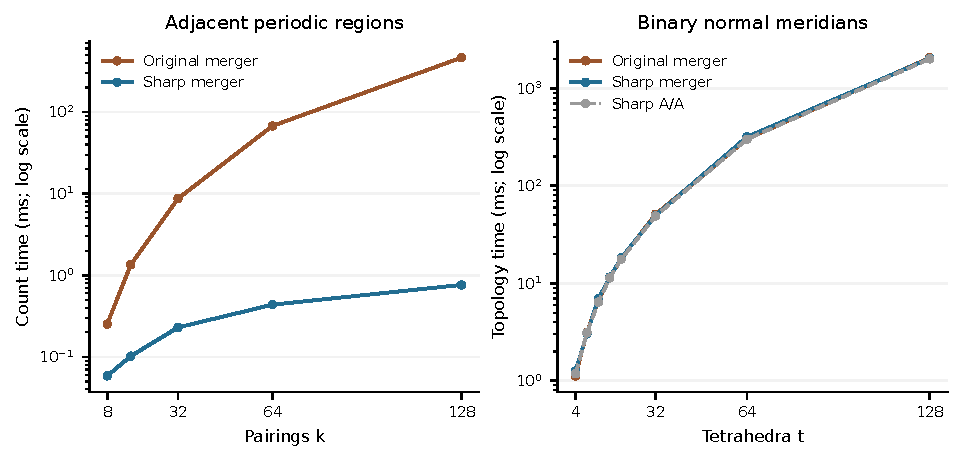
\includegraphics[width=\textwidth]{figures/interval_normal.pdf}
\caption{Measured local queries. Left: the adjacent periodic family with
$p=2^{512}+1$; points join the measured medians and do not represent a
fitted asymptotic law. Right: the complete native topology query for the
layered meridians, including validation and all three orbit counts.
Axes use logarithmic elapsed time. The normal-family curves do not show
a uniform timing advantage for the sharper merger.}
\label{fig:normal}
\end{figure}

The general AHT adapter should not replace the inherited specialized
extreme-ray disc check on the assumption that it will always be faster.
That check can be substantially cheaper on a primitive extreme-ray
meridian. The new adapter answers a broader question: it accepts arbitrary
admissible normal vectors and handles disconnected and one-sided surfaces.
The benchmark also scales a fixed meridian by powers of two through
$2^{2000}$ and verifies the resulting component count exactly. These
large-scale checks are supplementary correctness cases, not a timed
benchmark with repeated samples.

\subsection{Scalar equations on constructed and natural inputs}

Two kinds of valid homogeneous two-term algebraic complexes expose the
coefficient reduction. The sparse family uses two morphism coefficients
and field blocks of degree $d$. At $d=10$ it has 40 objects and 800 original
scalar variables, within the existing default admission cap. Forest
substitution leaves 400 variables. All arms recover the same
20-dimensional full commutant and the same complete compressed complex.
The experiment includes the cost of lifting and canonicalizing the basis.

\begin{table}[htbp]
\centering\small
\setlength{\tabcolsep}{4pt}
\begin{tabular}{@{}rrrrrrr@{}}
\toprule
$d$ & Objects & Direct ms & Span ms & Forest ms & Direct/forest & A/A\\\midrule
4 & 16 & 1.232 & 1.217 & 1.250 & 0.985 & 1.012\\
8 & 32 & 7.423 & 6.051 & 5.553 & 1.305 & 0.957\\
10 & 40 & 12.625 & 10.207 & 9.660 & 1.317 & 1.000\\
\bottomrule
\end{tabular}
\caption{Sparse two-field algebraic family: complete compression-pass medians.}
\label{tab:sparse}
\end{table}


The dense family keeps 16 objects and 128 original variables fixed.
Its two independent homogeneous coefficients partition the degree
$\lfloor b/2\rfloor$ dot monomials according to a chosen variable.
The actual coefficient rank is two, although an ambient coefficientwise
expansion generates thousands of equations. At $b=12$, the equation count
drops from 59\,136 to 128 under span reduction, and to 64 after the forest
substitution. The forest has 64 remaining variables. Table~\ref{tab:dense}
includes the entire compression pass, not merely Gaussian elimination.

\begin{table}[htbp]
\centering\small
\setlength{\tabcolsep}{4pt}
\begin{tabular}{@{}rrrrrrr@{}}
\toprule
$b$ & Direct equations & Span equations & Direct ms & Span ms & Direct/span & A/A\\\midrule
8 & 4480 & 128 & 12.856 & 2.000 & 6.530 & 0.994\\
10 & 16128 & 128 & 60.286 & 4.111 & 14.666 & 0.972\\
12 & 59136 & 128 & 516.973 & 12.815 & 38.521 & 0.996\\
\bottomrule
\end{tabular}
\caption{Dense homogeneous coefficients: equations and complete compression timings. Every row has 128 original variables; the forest has 64 variables and 64 equations.}
\label{tab:dense}
\end{table}


\begin{figure}[htbp]
\centering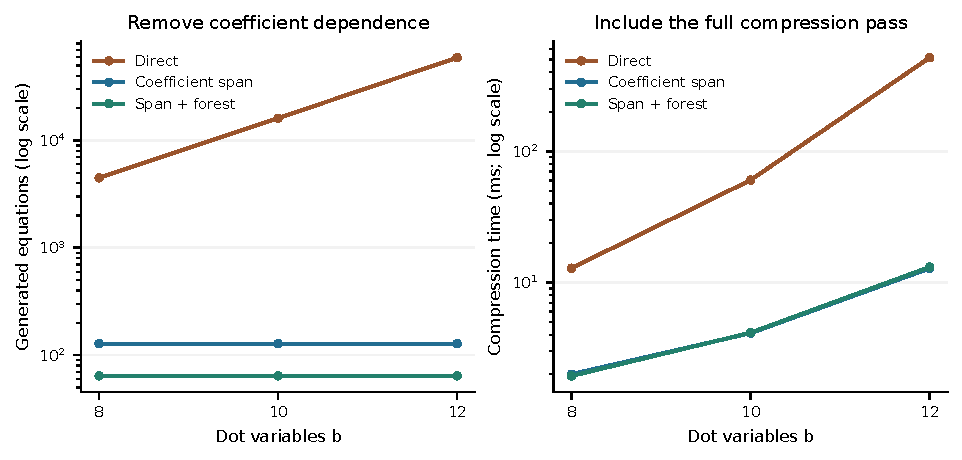
\includegraphics[width=\textwidth]{figures/scalar_coefficients.pdf}
\caption{Constructed homogeneous algebraic family, with no claimed
classical-knot realization. Left: generated scalar equation counts.
Right: complete compression-pass medians, including basis reconstruction.
The ambient coefficient values are still packed binary integers; their
bit length is part of the input and is not treated as constant.}
\label{fig:scalar}
\end{figure}

These are mathematically valid chain-complex examples, checked for
$D^2=0$ and grading consistency. They demonstrate an avoidable ambient
coefficient factor. They do not demonstrate that natural knot prefixes
attain this gap, nor polynomial time in $b$: the packed input itself can
have length exponential in the number of dot variables.

The natural-knot experiment freezes real scalar-solve inputs from three
scans. Summed across their eligible prefix solves, it finds the reductions
in Table~\ref{tab:natural_counts}. ``Remaining variables'' refers to the
reduced equation system; every returned basis is still expressed in the
full original variable space.

\begin{table}[htbp]
\centering\small
\setlength{\tabcolsep}{4pt}
\begin{tabular}{@{}lrrrrrr@{}}
\toprule
Input & Solves & Direct eq. & Span eq. & Forest eq. & $V$ & $V_F$\\\midrule
Conway & 10 & 1310 & 853 & 643 & 590 & 403\\
Kinoshita--Terasaka & 9 & 1324 & 905 & 699 & 551 & 362\\
5-braid stress (36) & 5 & 237 & 194 & 93 & 97 & 35\\
\bottomrule
\end{tabular}
\caption{Actual prefix commutants: sums of per-solve counts, not one simultaneous system.}
\label{tab:natural_counts}
\end{table}


Activation is therefore real. Nevertheless, the complete raw homology
scans in Table~\ref{tab:scans} show no consistent speedup. These scans run
the selected Khovanov backend directly, bypassing earlier recognition
filters so that they actually exercise its scalar machinery. They are
not full recognition-pipeline timings. No ordering search is included
in the timed calls; all arms use the same precomputed order, and their
graded homology agrees with the ordinary exact reference scan.

\begin{table}[htbp]
\centering\small
\setlength{\tabcolsep}{4pt}
\begin{tabular}{@{}lrrrrrr@{}}
\toprule
Input & Direct ms & Span ms & Forest ms & D/span & D/forest & A/A\\\midrule
Conway & 7.917 & 8.294 & 8.864 & 0.959 & 0.851 & 0.970\\
Kinoshita--Terasaka & 8.606 & 9.177 & 9.836 & 0.938 & 0.887 & 1.024\\
Hard unknot (8) & 0.713 & 0.757 & 0.715 & 1.017 & 0.949 & 0.925\\
5-braid stress (36) & 453.776 & 454.439 & 451.814 & 1.000 & 1.055 & 1.059\\
$T(3,5)$ & 3.062 & 3.000 & 2.865 & 1.026 & 1.037 & 1.044\\
\bottomrule
\end{tabular}
\caption{Complete raw homology scans with identical scan order and graded answer. Ratios are median paired ratios. Values near one should be read alongside the A/A control.}
\label{tab:scans}
\end{table}


Transport overhead, small original systems and work elsewhere in the scan
can absorb the reduced solve cost. The maintained default consequently
remains \code{direct}; \code{span} and \code{forest} are explicit options.
A blanket recommendation to enable forest reduction on every prefix
would go beyond these measurements.

\subsection{Whole knot queries and the explicit overlap kernel}

The relator corpus contains twelve maintained survivor unknot diagrams,
two of their mirrors, the 141-crossing Gordian unknot, and four nontrivial
controls. Each is run with the explicit and the compressed group-search
configuration. Four arms compare the historical pairwise query, its A/A
copy, the new adaptive query and the shared index alone. All 760 measured
whole queries, together with 152 excluded warmups, complete with the
expected result. No censored or inconclusive result is silently converted
to a successful timing. Full PD encodings, configurations, status records
and certificate hashes are included in the raw JSON.

\begin{table}[htbp]
\centering\small
\setlength{\tabcolsep}{4pt}
\begin{tabular}{@{}lrrrrrr@{}}
\toprule
Search mode & Pairwise ms & Adaptive ms & Joint ms & P/adaptive & P/joint & A/A\\\midrule
explicit & 830.706 & 490.701 & 931.036 & 1.766 & 0.920 & 1.068\\
compressed & 1357.319 & 1045.271 & 1487.001 & 1.297 & 0.911 & 1.008\\
\bottomrule
\end{tabular}
\caption{Complete configured Gordian recognition queries, including independent replay. The explicit-query replacement can also be reached inside the configured compressed route.}
\label{tab:gordian}
\end{table}


The Gordian improvement is attributable to one residual overlap query,
after 129 generator eliminations. It has twelve nonempty relators of
total length 17\,504. The maximum guaranteed gain is 2\,998, and the
adaptive prelude needs four oriented donor automata in place of 24.
The selected move and the complete 141-move certificate are unchanged on
this input. The independent replay modules do not use the producer's
shared index. Tests also disable producer-only helpers during replay,
so accepting the optimized search output is not circular.

The shared index by itself regresses on Gordian. This negative arm is
retained in the table. Its larger construction cost is justified for
many relators, whereas Gordian admits strong incumbent bounds early.
The fixed four-relator base case avoids paying a failed prelude followed
by shared construction on very small lists. The initial measurement run,
which motivated that base case, is retained separately as calibration
data together with the matching index source; it is not mixed into the
final medians.

\begin{table}[htbp]
\centering\small
\setlength{\tabcolsep}{4pt}
\begin{tabular}{@{}lrrrrrr@{}}
\toprule
Input & $\ell$ & Gain & Pairwise ms & Adaptive ms & Joint ms & P/adaptive\\\midrule
Gordian residual & 17504 & 2998 & 265.052 & 62.032 & 416.868 & 4.232\\
$8\times64$ random & 512 & 0 & 8.249 & 9.809 & 7.025 & 0.859\\
$32\times64$ random & 2048 & 0 & 129.521 & 46.800 & 26.003 & 2.768\\
$128\times64$ random & 8192 & 0 & 2066.899 & 231.601 & 185.595 & 8.798\\
Periodic duplicates & 32768 & 1024 & 74.049 & 4.485 & 311.439 & 16.510\\
\bottomrule
\end{tabular}
\caption{Exact explicit overlap queries, including all index construction and any failed prelude. Only the first row comes from the measured knot presentation; the others are synthetic capacity cases.}
\label{tab:overlap_kernels}
\end{table}


The random relator rows are exact-query capacity experiments, not knot
recognition results. Their optimum gain is zero, so a correct query must
rule out every eligible shortening. On the 128-by-64 case the simultaneous
index removes the repeated target scans, and the adaptive route retains
most of the benefit even after charging its failed prelude. The eight-by-64
case is a counterexample to universal practical improvement: the adaptive
query can be slower. Highly repetitive duplicate relators favor early
donor bounds, again making the adaptive route preferable to always
building the shared index. No single timing arm is best on every row.

\subsection{Independent correctness and validation coverage}

The mathematical specifications are checked by several different oracles.
The interval suite compares both merger policies with literal disjoint-set
connectivity on 9\,882 small two-pairing systems, exhaustive tiny triples
and 2\,000 randomized systems. It exhausts the relevant two-period
thresholds for periods through twelve, checks invalid endpoints and
shared budgets, and includes 700 independently counted signed systems.
Large integer tests ensure that bit length, rather than represented
interval size, determines storage.

The normal-surface suite checks explicit arc graphs, reoriented and
relabelled triangulations, the zero surface, vertex-linking discs,
essential meridians and one-sided M\"obius families. It compares normal
surfaces and compatible sums in small layered triangulations against
Regina 7.4 for connected components, orientability, boundary count, Euler
characteristic and compressing-disc status \cite{regina}. It also compares
the native ambient validator against Regina on the enumerated one-face
gluing cases. Regina is an optional independent test dependency; neither
new production module imports it.

The scalar suite reconstructs coefficient entries, exhausts 256 small
two-coefficient matrix systems, checks randomized rectangular blocks and
compares the canonical complete nullspace in all modes. It verifies
actual split witnesses, static child-commutant reuse and the existing
admission caps. These tests establish equality of the object used by the
bounded candidate policy, not just equality of nullity.

The overlap suite checks 7\,056 exhaustive small ordered word pairs,
350 small multisets against a literal all-rotation oracle, and 600 larger
multisets against the historical query. Cases include inverse donors,
periodic words, zero-length slots, equal words in distinct slots, cap
boundaries, cancellation, malformed witnesses and tampered certificates.
The exhaustive and differential comparisons require the same optimal
gain and a valid attaining witness; the general shared index is allowed
to choose a different tied witness. Complete corpus certificates are
also compared explicitly.

\paragraph{Full integration gate.}
With the pinned sibling reference dependencies restored, the untouched
baseline runs 768 test methods: 767 pass and one fails with the inherited
delayed-input subprocess timeout. The maintained overlay passes all
\textbf{807 test methods}, with no failures, errors or skips. The integrated
run includes the repaired worker regression and 39 additional test methods;
many methods contain large exhaustive or randomized families. The baseline
and maintained runs report 112.659 and 120.692 seconds respectively. These
different-size suite durations are validation records, not a performance
comparison. Source hashes are unchanged throughout both runs, and the
446-file baseline staging archive remains byte-identical. Full logs and a
machine-readable summary accompany the article.

